%! TeX program = lualatex
\documentclass[a4paper,11pt]{report}
% packages
\usepackage{censor}
\StopCensoring
\usepackage{fontspec}
\setmainfont{EB Garamond}
% for tironian et fallback
% % \directlua{luaotfload.add_fallback
% % ("emojifallback",
% %      {"Noto Serif:mode=harf"}
% % )}
% % \setmainfont{EB Garamond}[RawFeature={fallback=emojifallback}]

\setmonofont[Scale=MatchLowercase]{Deja Vu Sans Mono}
\usepackage[a4paper,left=2cm,right=2cm,top=\dimexpr15mm+1.5\baselineskip,bottom=2cm]{geometry}
\setlength{\parindent}{0pt}

\usepackage{fancyhdr}       % Headers and footers 
\fancyhead[R]{\normalfont \leftmark}
\fancyhead[L]{}
\pagestyle{fancy}

\usepackage{microtype}      % Slightly tweak font spacing for aesthetics
\usepackage[english]{babel} % Language hyphenation and typographical rules
\usepackage{xcolor}
\definecolor{linkblue}{RGB}{0, 64, 128}
\usepackage[final, colorlinks = false, urlcolor = linkblue]{hyperref} 
% \newcommand{\secref}[1]{\textbf{§~\nameref{#1}}}
\newcommand{\secref}[1]{\textbf{§\ref{#1}~\nameref{#1}}}

\usepackage{changepage}     % adjust margins on the fly
\usepackage{amsmath}
\usepackage{amsmath,amssymb}

\usepackage[backend=biber, style=numeric, date=iso, urldate=iso]{biblatex}
\addbibresource{references.bib}
\DeclareFieldFormat{urldate}{Accessed on: #1}

\usepackage{minted}
\usemintedstyle{algol_nu}

\usepackage{pgfplots}
\pgfplotsset{width=\textwidth,compat=1.9}

\usepackage{caption}
\newenvironment{code}{\captionsetup{type=listing}}{}
\captionsetup[listing]{skip=0pt}
\setlength{\abovecaptionskip}{5pt}
\setlength{\belowcaptionskip}{5pt}

\usepackage[yyyymmdd]{datetime}
\renewcommand{\dateseparator}{--}

\usepackage{enumitem}

\usepackage{titlesec}

\author{Andrew Hayes}

\begin{document}
\begin{titlepage}
    \begin{center}

        % University Logo
        
\includegraphics[width=0.8\textwidth]{./images/Logo-UGalway-2-3166136658.jpg} \\[1cm]

        % Title
        {\Huge \textbf{Iompar: Live Public Transport Tracking}} \\[0.5cm]
        
        % Department and Degree
        {\Large College of Science \& Engineering} \\[0.3cm]
        {\large Bachelor of Science (Computer Science \& Information Technology)} \\[0.5cm]

        % Report Type
        {\large \textbf{Project Report}} \\[1.5cm]

        % Author Section
        {\Large \textbf{Author:}} \\[0.2cm]
        {\large Andrew Hayes \\ 21321503 } \\[1cm]

        % Supervisor Section
        {\Large \textbf{Academic Supervisor:}} \\[0.2cm]
        {\large Dr. Adrian Clear} \\[1.5cm]

        % Date
        {\Large \today}

    \end{center}
\end{titlepage}

\pagenumbering{roman}
\newpage
\tableofcontents
\newpage
\setcounter{page}{1}
\pagenumbering{arabic}

% yap about mental models with regards to how filters work
% trying to make the application work the same way the user expects it to work

\chapter{Introduction}
\section{Project Overview}
\subsection{Problem Statement}
\subsection{Background}
\section{Document Structure}

\chapter{Research}
\section{Introduction}
\section{Data Sources}
\section{Similar Services}
\section{Technologies}
\subsection{Frontend Technologies}
\subsection{Backend Technologies}
\subsection{Project Management Technologies}
\section{Conclusion}

\chapter{Requirements}
\section{Functional Requirements}
\section{Non-Functional Requirements}
\section{Use Cases}
\section{Constraints}

\chapter{Design}
\section{Backend Design}
\begin{figure}[H]
    \centering
    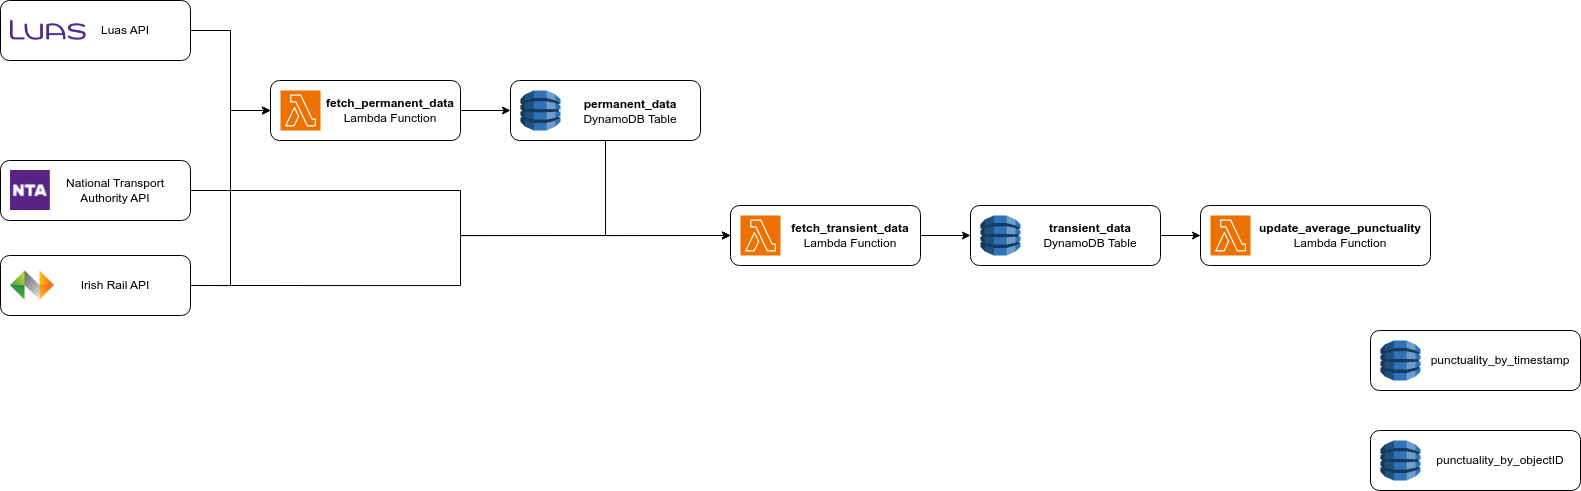
\includegraphics[width=\textwidth]{./images/diagram_all.png}
    \caption{Backend architecture}
\end{figure}

\subsection{Database Design}
Since the chosen database system was DynamoDB, a No-SQL database, the question of how best to separate the data is more open-ended: unlike a relational database, there is no provably correct, optimised structure of separated tables upon which to base the database design.
The decision was made that data would be separated into tables according to the type of data, how its used, and how its updated, thus allowing separation of concerns for functions which update the data and allowing different primary keys and indices to be used for different querying patterns.

\subsubsection{Permanent Data Table}
The permanent data table holds the application data which is unchanging and needs to be updated only rarely, if ever.
This includes information about bus stops, train stations, Luas stops, and bus routes.
This data does not need to be updated regularly, just on an as-needed basis.
Since this data is not temporal in nature, no timestamping of records is necessary.

\begin{code}
\begin{minted}[linenos, breaklines, frame=single]{json}
[
  {
    "objectID": "IrishRailStation-GALWY",
    "objectType": "IrishRailStation",
    "trainStationCode": "GALWY",
    "trainStationID": "170",
    "trainStationAlias": null,
    "trainStationDesc": "Galway",
    "latitude": "53.2736"
    "longitude": "-9.04696",
  },
  {
    "objectID": "BusStop-8460B5226101",
    "objectType": "BusStop",
    "busStopID": "8460B5226101",
    "busStopCode": "522611",
    "busStopName": "Eyre Square",
    "latitude": "53.2750947795551"
    "longitude": "-9.04963289544644",
  },
  {
    "objectID": "BusRoute-4520_67654",
    "objectType": "BusRoute",
    "busRouteID": "4520_67654"
    "busRouteAgencyName": "City Direct",
    "busRouteAgencyID": "7778028",
    "busRouteShortName": "411",
    "busRouteLongName": "Mount Prospect - Eyre Square",
  },
  {
    "objectType": "LuasStop",
    "objectID": "LuasStop-STS",
    "luasStopCode": "STS"
    "luasStopID": "24",
    "luasStopName": "St. Stephen's Green",
    "luasStopIrishName": "Faiche Stiabhna",
    "luasStopIsParkAndRide": "0",
    "luasStopIsCycleAndRide": "0",
    "luasStopLineID": "2",
    "luasStopZoneCountA": "1",
    "luasStopZoneCountB": "1",
    "luasStopSortOrder": "10",
    "luasStopIsEnabled": "1",
    "latitude": "53.3390722222222",
    "longitude": "-6.26133333333333",
  }
]
\end{minted}
\caption{Sample of the various types of items stored in the permanent data table}
\end{code}

Beyond what is returned for an item by its source API, two additional fields are included for each item:
the \verb|objectType| to allow for querying based on this attribute and the \verb|objectID|, an attribute constructed from an item's \verb|objectType| and the unique identifier for that item in the system from which it was sourced, thus creating a globally unique identifier for the item.
However, this attribute is \textit{not} used as the primary key for the table;
instead, it exists primarily so that each item has a unique identifier that does not need to be constructed on the fly on the frontend, thus allowing the frontend to treat specific items in specific ways.
An example of a use for this is the ``favourites'' functionality: a unique identifier must be saved for each item that is added to a user's favourites.
Defining this unique identifier in the backend rather than the frontend reduces frontend overhead (important when dealing with tens of thousands of items) and also makes the system more flexible.
While the ``favourites'' functionality is implemented fully on the frontend at present, the existence of unique identifiers for items within the table means that this functionality could be transferred to the backend without major re-structuring of the database.
\\\\
There are two ways in which a primary key can be created for a DynamoDB table\supercite{choosing-the-right-key}:
\begin{itemize}
    \item   A simple primary key, consisting solely of a \textbf{partition key}: the attribute which uniquely identifies an item, analogous to simple primary keys in relational database systems.

    \item   A composite primary key, consisting of a partition key and a \textbf{sort key}, analogous to composite primary keys in relational database systems.
            Here, the partition key determines the partition in which an item's data is stored, and the sort key is used to organise the data within that partition.
\end{itemize}

While the \verb|objectID| could be used as a partition key and thus a simple primary key, it was decided not to use the attribute for this purpose as it was not the most efficient option.
The primary function of the permanent data table is to provide data for a user when they want to display a certain type of object, such as bus stops, train stations, Luas stops, or some combination of the three.
Therefore, the most common type of query that the table will be dealing with is queries which seek to return all items of a certain \verb|objectType|.
Partitioning the table by \verb|objectID| would make querying by \verb|objectID| efficient, but all other queries inefficient, and querying by \verb|objectID| is not useful for this application.
Instead, the permanent data table uses a composite primary key, using the \verb|objectType| as the partition key and the \verb|objectID| as the sort key.
Thus, it is very efficient to query by \verb|objectType| and return, for example, all the bus stops and Luas stops in the country.
\\\\
Technically speaking, there is some redundant data in each primary by using the \verb|objectID| as the sort key when the partition key is the \verb|objectType|: since the \verb|objectID| already contains the \verb|objectType|, it is repeated.
However, the unique identifier for each item is different depending on the system from which it was sourced:
for train stations, the unique identifier is named \verb|trainStationCode|, while the unique identifier for bus stops is named \verb|busStopID|.
To use these fields as sort key, they would have to be renamed in each item to some identical title, thus adding overhead to the process of fetching data, and making the table less human-readable.
Since the \verb|objectID| was to be constructed regardless for use on the frontend, it is therefore more efficient to re-use it as the sort key, even if it does result in a few bytes of duplicated data in the primary key of each item.

% The primary key of this table is the \verb|objectID|, necessarily unique to each record in the table.
% This is constructed as a combination of the \verb|objectType| (e.g., \verb|BusStop|, \verb|IrishRailStation|) and the unique identifier for that object returned by the API from which the data was retrieved.
% The prefix of the \verb|objectType| is used here to guarantee uniqueness of the primary key in the case that two objects in the table of differing types have the same ID given to them by their respective source APIs.
% \\\\
% There are two ways in which a primary key can be created for a DynamoDB table\supercite{choosing-the-right-key}:
% \begin{itemize}
%     \item   A simple primary key, consisting solely of a \textbf{partition key}: the attribute which uniquely identifies an item, analogous to simple primary keys in relational database systems.
%
%     \item   A composite primary key, consisting of a partition key and a \textbf{sort key}, analogous to composite primary keys in relational database systems.
%             Here, the partition key determines the partition in which an item's data is stored, and the sort key is used to organise the data within that partition.
% \end{itemize}
%
% Instead of constructing a new attribute \verb|objectID| for an item, it would also be possible to avoid creating a new attribute by instead using a composite primary key, with the partition key being the item's unique identifier in the system from which it came and the sort key being the \verb|objectType|.
% This was rejected in favour of constructing a new attribute, \verb|objectID| to serve as the simple primary key for this table for a number of reasons:
% \begin{itemize}
%     \item   The uniquely identifying attribute for each item given to it by the API from which said item was sourced has a different attribute name for every API;
%             the unique identifier for bus stops is \verb|busStopID|, for train stations is \verb|trainStationCode|, et cetera.
%             To use these values as the primary key in the table, each of these attributes would have to be re-named to some single, unifying title, creating additional parsing overhead when the data is being uploaded to the table, and making the item information more difficult to read for humans.
%
%     \item   Having a single uniquely identifying attribute for each item is useful on the frontend, allowing items to be easily uniquely identified without additional processing, useful for user functionality such as adding an item to the user's ``favourites''.
%
%     \item   The query efficiency improvements typically associated with a DynamoDB composite key would not apply to the type of queries this table is designed for with such a composite key structure.
%             The data from this table will most often be queried by \verb|objectType| in this application, such as in the event that a user wants to see bus stops or train stations or both on a map.
%             The composite key would only speed up querying in the event that, for a number of different items with the same unique identifier, a query was ran on based on the type of those objects sharing an identifier, which is not a situation that is likely to arise for this application.
% \end{itemize}
%
% As mentioned in the final bullet-point above, this table is only intended for a single type of query:
% queries which seek to return all the items in the table of a certain \verb|objectType| or \verb|objectType|s, such as when a frontend user requests to see bus stops, or train stations, or Luas stops, or some combination of the three.
% Therefore, it is imperative that such queries are efficient \& fast. 
% Since we cannot partition the data 

\subsubsection{Transient Data Table}
The transient data table holds the live tracking data for each currently running public transport vehicle in the country, including information about the vehicle and its location.
Similar to the permanent data table, a unique \verb|objectID| is constructed for each item.

\begin{code}
\begin{minted}[linenos, breaklines, frame=single]{json}
[
  {
    "objectType": "IrishRailTrain",
    "latenessMessage": "On time",
    "timestamp": "1742897696",
    "trainDirection": "Southbound",
    "trainStatus": "R",
    "trainDetails": "09:41 - Maynooth to Grand Canal Dock ",
    "trainType": "S",
    "objectID": "IrishRailTrain-P656",
    "averagePunctuality": "0",
    "trainUpdate": "Departed Pelletstown next stop Broombridge",
    "trainStatusFull": "Running",
    "longitude": "-6.31388",
    "trainPublicMessage": "P656\\n09:41 - Maynooth to Grand Canal Dock (0 mins late)\\nDeparted Pelletstown next stop Broombridge",
    "trainPunctuality": "0",
    "trainPunctualityStatus": "on-time",
    "trainTypeFull": "Suburban",
    "trainDate": "25 Mar 2025",
    "latitude": "53.3752",
    "trainCode": "P656"
  },
  {
    "objectType": "Bus",
    "busScheduleRelationship": "SCHEDULED",
    "timestamp": "1742908007",
    "busID": "V598",
    "busRoute": "4538_90219",
    "busRouteAgencyName": "Bus Éireann",
    "objectID": "Bus-V598",
    "busRouteLongName": "Galway Bus Station - Derry (Magee Campus Strand Road)",
    "longitude": "-8.50166607",
    "busDirection": "1",
    "busStartDate": "20250325",
    "busRouteShortName": "64",
    "latitude": "54.2190742",
    "busTripID": "4538_114801",
    "busStartTime": "10:30:00"
  },
\end{minted}
\caption{Sample of the various types of items stored in the transient data table}
\end{code}

There are only two types of objects stored in the transient data table: Irish Rail Trains and Buses.
There is no per-vehicle data provided in the Luas API, and thus no way to track the live location of Luas trams.
For the two types of objects stored in the transient data table, additional fields are added beyond what is returned by their respective APIs (and beyond the \verb|objectType| \& \verb|objectID| fields) to augment the data.
\\\\
The following additional pieces of data are added to each \verb|IrishRailTrain| object:
\begin{itemize}
    \item   The \verb|trainStatus| \& \verb|trainType| fields are single-character codes returned by the API, representing longer strings; for example a \verb|trainStatus| of \verb|"R"| indicates that the train is \textit{running}.
            To avoid having to construct these strings on the frontend, the fields \verb|trainStatusFull| \& \verb|trainTypeFull| are automatically added to the record when the data is retrieved.

    \item   The Irish Rail API compacts much of its interesting data into a single field: \verb|trainPublicMessage|.
            This field contains the \verb|trainCode| (which is also supplied individually in its own field by the API), a string containing details about the train's origin \& terminus, a string describing how late the train is, a string containing an update about the train's current whereabouts, all separated by \verb|\\n| characters.
            This string is parsed into several additional fields to prevent additional computation on the frontend, including:
            \begin{itemize}
                \item   \verb|latenessMessage|: a human-readable string which describes whether a train is early, late, or on time.
                \item   \verb|trainDetails|: a string describing the train service itself, its start time, origin, \& terminus.
                \item   \verb|trainUpdate|: a string containing an update about the current whereabouts of the train, such as what station it last departed and what station it will visit next. 
                \item   \verb|trainPunctuality|: an integer which represents how many minutes late the train is (where a negative number indicates that the train is that many minutes early).
                \item   \verb|trainPunctualityStatus|: a whitespace-free field which gives the same information as \verb|latenessMessage| but for use in filtering rather than information presentation to the user.
                        While one of these fields could be derived from the other on the frontend, the extra computation necessary when repeated for multiple trains and multiple users dwarfs the few extra bytes in the database to store the data in the machine-readable and human-readable forms.
            \end{itemize}

    \item   The \verb|averagePunctuality| field is a field which contains the average recorded value of the \verb|trainPunctuality| for trains with that \verb|trainCode| in the database, thus giving a predictor of how early or late that particular train usually is.
\end{itemize}

The following additional pieces of data are added to each \verb|Bus| object:
\begin{itemize}
    \item   \verb|busRouteAgencyName|.
    \item   \verb|busRouteShortName|.
    \item   \verb|busRouteLongName|.
\end{itemize}

These details are not included in the response from the GTFS API, but can be obtained by looking up the given \verb|busRoute| attribute in the permanent data table to find out said information about the bus route.
In a fully-normalised relational database, this would be considered data duplication, but storing the data in both places allows for faster querying as no ``joins'' need to be performed.
\\\\
Since the primary role of the transient data table is to provide up-to-date location data about various public transport services, each item in the table is given a \verb|timestamp| attribute.
This \verb|timestamp| attribute is a UNIX timestamp in seconds which uniquely identifies the batch in which this data item was obtained.
Each train \& bus obtained in the same batch have the same \verb|timestamp|, making querying for the newest data in the table more efficient.
Because the data is timestamped, old data does not have to be deleted, saving both the overhead of deleting old data every time new data is fetched, and allowing an archive of historical data to be built up over time. 
\\\\
Since the primary type of query ran on this table will be queries which seek to return all the items of a certain \verb|objectType| (or \verb|objectType|s) for the latest timestamp, it would be ideal if the primary key could be a combination of the two for maximum efficiency in querying;
however, such a combination would fail to uniquely identify each record and thus would be inappropriate for a primary key.
Instead, the primary key must be some combination of the \verb|timestamp| attribute and the \verb|objectID| attribute.
It was decided that the partition key would be the \verb|objectID| and the sort key to be the \verb|timestamp| so that all the historical data for a given item could be retrieved efficiently.
Equivalently, the partition key could be the \verb|timestamp| and the sort key could be the \verb|objectID| which would allow for queries of all items for a given timestamp, but this was rejected on the basis that such scenarios were covered by the introduction of a Global Secondary Index.
\\\\
A \textbf{Global Secondary Index (GSI)} allows querying on non-primary key attributes by defining an additional partition and sort key from the main table\supercite{gsi}.
Unlike a primary key, there is no requirement for a GSI to uniquely identify each record in the table;
a GSI can be defined on any attributes upon which queries will be made.
The addition of GSIs to a table to facilitate faster queries is analogous to \mintinline{sql}{SELECT} queries on non-primary key columns in a relational database (and the specification of a sort key is analogous to a relational \mintinline{sql}{ORDER BY} statement);
the structured nature of a relational database means that such queries are relatively efficient by default as each column in the table functions as an index itself.
In a No-SQL database, this functionality does not come for free, and instead must be manually specified.
\\\\
To facilitate efficient querying of items in the table by \verb|objectType| and \verb|timestamp|, a GSI was created with partition key \verb|objectType| and sort key \verb|timestamp|, thus making queries for the newest data on a public transport type as efficient as querying on primary key attributes.
The downside of creating a GSI is the additional storage requirements, as DynamoDB implements GSIs by duplicating the data into a separate index: efficient for querying, but less so in terms of storage usage.

\subsubsection{Average Punctuality by \texttt{objectID} Table}
To give the user punctuality predictions based off the historical data stored for a given service, it's necessary that the average punctuality be calculated.
The most obvious way to do this would be to calculate the average of the punctuality values for a given \verb|objectID| in the transient data table every time data a new data item with that \verb|objectID| is added to the transient data table.
However, this would be greatly inefficient, as it would require scanning the entire table for each item uploaded to the table, greatly slowing down the fetching of new data and consuming vast amounts of DynamoDB read/write resources.
It is also intractable, as the historical data archive in the transient table grows, it will become linearly more expensive to compute the average punctuality for an item.
\\\\
Instead, it was decided that the average punctuality for an item would be stored in a table and updated as necessary.
By storing the \verb|objectID|, the \verb|average_punctuality|, and the \verb|count| of the number of records upon which this average is based, the mean punctuality for an item can be updated on an as-needed basis in an efficient manner.
The new mean value for an item can be calculated as:
\[
  \bar{x}_{\text{new}} = \frac{(\bar{x}_\text{old} \times c) + x}{c+1}
\]
where $x$ is the punctuality value for a given item, $\bar{x}_{\text{old}}$ is the previous mean punctuality value for that item, $c$ is the count of records upon which that mean was based, and $\bar{x}_{\text{new}}$ is the new mean punctuality value.
By calculating the average punctuality in this way, the operation is $O(1)$ instead of $O(n)$, thus greatly improving efficiency. 

\begin{code}
\begin{minted}[linenos, breaklines, frame=single]{json}
[
  {
    "average_punctuality": "0.5",
    "count": "2",
    "objectType": "IrishRailTrain",
    "objectID": "IrishRailTrain-P746"
  },
  {
    "average_punctuality": "-4",
    "count": "1",
    "objectType": "IrishRailTrain",
    "objectID": "IrishRailTrain-A731"
  },
  {
    "average_punctuality": "9.333333333333333333333333333",
    "count": "3",
    "objectType": "IrishRailTrain",
    "objectID": "IrishRailTrain-E112"
  },
]
\end{minted}
\caption{Sample of items from the average punctuality by \texttt{objectID} table}
\end{code}

At the time of writing, Irish Rail is the only Irish public transport provider to offer any kind of punctuality data in their public APIs, and therefore, this table only stores items with \mintinline{json}{"objectType": "IrishRailTrain"}.
It could be argued that including this value in the table is therefore redundant, as it can be inferred, but the decision was made to include this additional value to make the table expandable and updatable.
If another transport provider were to begin to offer punctuality data via their API, this table would require no updates to start including, for example, bus punctuality data.
If the \verb|objectType| were not included, this table would have to be replaced with a re-structured table in the event that a new category of public transport items were to be added.
\\\\
In the same vein as including the \verb|objectType| in each record, the primary key for this table was created with partition key \verb|objectType| and sort key \verb|objectID|, like in the permanent data table.
This means that if an additional type of public transport were to be added to the table, querying based on that \verb|objectType| would be fast \& efficient by default.
Since the primary key of a table cannot be changed once the table has been created, not using the \verb|objectType| in the primary key would meant that adding an additional public transport type to the table would require deleting the table and starting again, or at the very least the creation of an otherwise unnecessary GSI to facilitate efficient querying.

\subsubsection{Punctuality by \texttt{timestamp} Table}
To provide historical insights such as punctuality trends over time, it is necessary to keep a record of the average punctuality for each timestamp recorded in the database.
Similarly to the punctuality by \verb|objectID| table, it is more efficient to calculate this value and store it than to calculate the average for every item in the table as the data is needed.
Unlike the punctuality by \verb|objectID| table, however, the average punctuality value for a \verb|timestamp| need never be updated, as the average is calculated for each data upload run.

\begin{code}
\begin{minted}[linenos, breaklines, frame=single]{json}
[
  {
    "average_punctuality": "0.8823529411764706",
    "timestamp": "1742908007"
  },
  {
    "average_punctuality": "1.0625",
    "timestamp": "1742905796"
  }
]
\end{minted}
\caption{Sample of items from the average punctuality by \texttt{timestamp} table}
\end{code}

The partition key for this table is the \verb|timestamp| value, and there is no need for a sort key or secondary index.

\subsection{API Design}


\subsection{Serverless Functions}

\section{Frontend Design}

\chapter{Development}
\section{Introduction}
\section{Backend Development}
\section{Frontend Development}
\section{Development Considerations}

\chapter{Code Quality}
\section{Introduction}
\section{Clean Coding Principles}
\section{Unit Testing}
\section{CI/CD}
\subsection{Continuous Integration}
\subsection{Continuous Deployment}

\chapter{Conclusion}
\section{Evaluation}
\section{Reflection on Requirements}
\section{Reflection on Skill Development}
\section{Potential Future Work}

\printbibliography


\end{document}
